\documentclass[11pt]{scrartcl}
\usepackage[sexy]{evan}
\usepackage{graphicx}

\newcommand{\N}{\mathbb{N}}
\newcommand{\Z}{\mathbb{Z}}
\newcommand{\F}{\mathbb{F}}
\newcommand{\Q}{\mathbb{Q}}
\newcommand{\R}{\mathbb{R}}
\newcommand{\C}{\mathbb C}


\newcommand{\Vu}{\mathbf{u}}
\newcommand{\Vv}{\mathbf{v}}
\newcommand{\Vw}{\mathbf{w}}
\newcommand{\Vx}{\mathbf{x}}
\newcommand{\Ve}{\mathbf{e}}
\newcommand{\Vc}{\mathbf{c}}
\newcommand{\Vb}{\mathbf{b}}



\newcommand{\Va}{\mathbf{a}}

\newcommand{\Vhx}{\mathbf{\hat{x}}}

\newcommand{\Vy}{\mathbf{y}}
\newcommand{\Vz}{\mathbf{z}}
\newcommand{\Vo}{\mathbf{0}}

%From Topology
\newcommand{\cT}{\mathcal{T}}
\newcommand{\cB}{\mathcal{B}}
\newcommand{\cC}{\mathcal{C}}

\usepackage{answers}
\Newassociation{hint}{hintitem}{all-hints}
\renewcommand{\solutionextension}{out}
\renewenvironment{hintitem}[1]{\item[\bfseries #1.]}{}
\declaretheorem[style=thmbluebox,name={Theorem}]{thm}

\begin{document}
\title{CS 189}
\author{Vishal Raman}

\section{Homework 6: Convolutions and Transformers}
“I certify that all solutions are entirely in my own words and that I have not looked at another student’s solutions. I have given credit to all external sources I consulted.
\subsection{Problem I}
\begin{itemize}
\item[(a)] We have $(4 \cdot 1 + 1) \cdot 8 = 40$ parameters.  The output tensor has size $\frac{(200 - 4 + 2 \cdot 0)}{2} \times 1= 98 \times 1.$

\item[(b)] We have $(4 \cdot 4 \cdot 3 + 1) \cdot 8 = 392$.   parameters. The size of the output tensor is given by $$\frac{(28 - 4 + 2 \cdot 0)}{2} \times \frac{(28 - 4 + 2 \cdot 0)}{2} \times 3 = 12 \times 12 \times 3.$$

\item[(c)]  The result of average pooling for each matrix is given by 
$$\begin{bmatrix}
\frac{8}{9} & \frac{2}{3} \\
\frac{2}{3} & \frac{5}{9}
\end{bmatrix},
\begin{bmatrix}
\frac{1}{3} & \frac{1}{3} \\
\frac{1}{3} & \frac{1}{3}
\end{bmatrix}.
$$

The result of max pooling for each matrix is given by 
$$\begin{bmatrix}
1 & 1 \\
1 & 1
\end{bmatrix},
\begin{bmatrix}
1 & 1\\
1 & 1
\end{bmatrix}.
$$
\item[(d)] In the case of max pooling, since we have a small amount of noise, we can perform analysis on the pooled where each cell corresponds to the maximum value in a corresponding block.   We also take advantage of the convolutional structure which has translational invariance and spatial locality.  The case with average pooling is similar - with small distortions, we can take the average within blocks and perform analysis on the corresponding pooled tensor.
\end{itemize}

\newpage

\subsection{Problem II}
\begin{itemize}
\item[(a)] The images are $28 \times 28$.  The values are in the range $[0, 1]$ and correspond to the gray-scale opacity of the corresponding pixel - $0.0$ corresponds to black, $1.0$ corresponds to white, and they scale continuously in between these values.  There are $48000$ images in the training set.  There are $10000$ images in the test set.  
\item[(b)]
\begin{center}
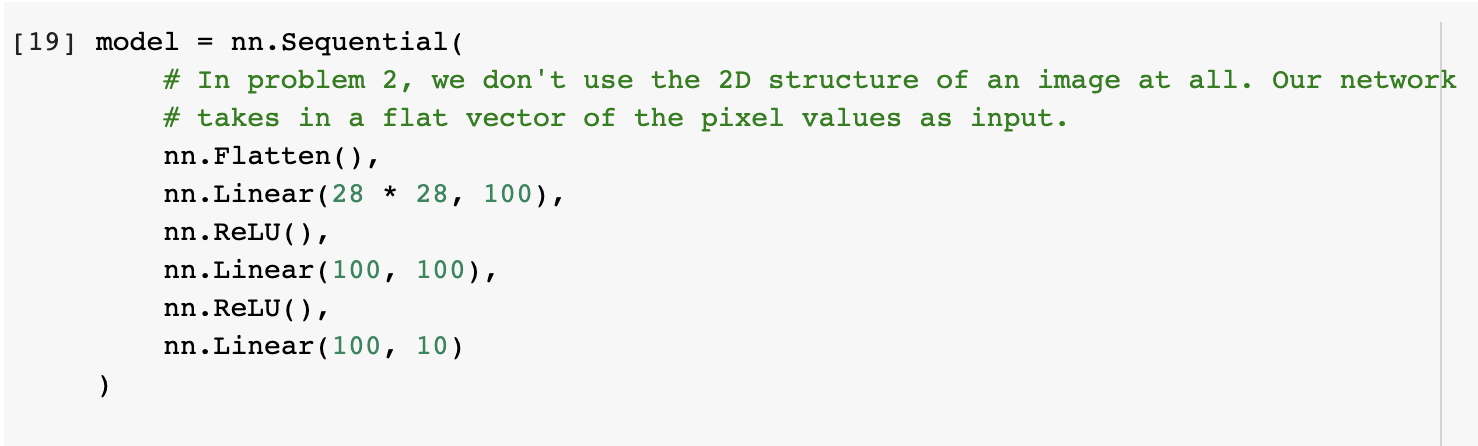
\includegraphics[scale=0.5]{model.png}
\end{center}

\begin{center}
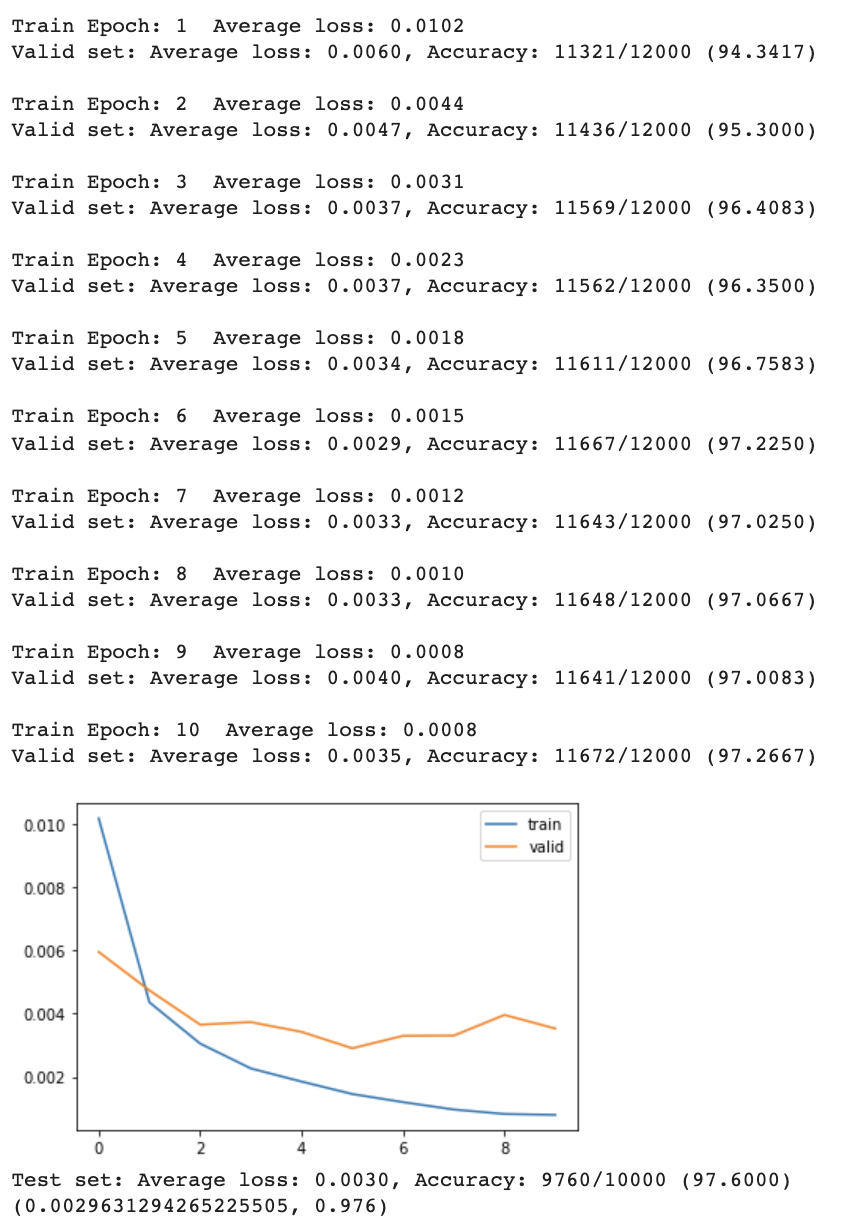
\includegraphics[scale=0.5]{results.png}
\end{center}

The first model I used worked using the default batch and epoch size.  I essentially stacked two of the default linear models together, using a larger number of hidden layers.

\item[(c)]
\begin{center}
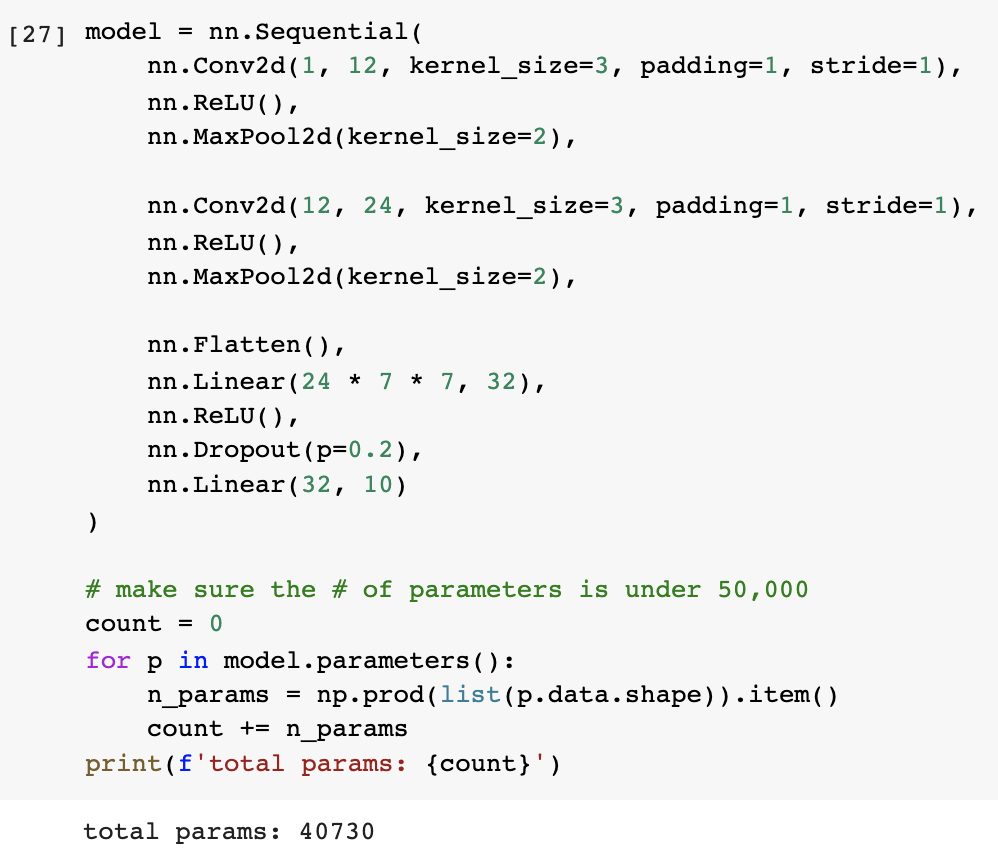
\includegraphics[scale=0.5]{convModel.png}
\end{center}

\begin{center}
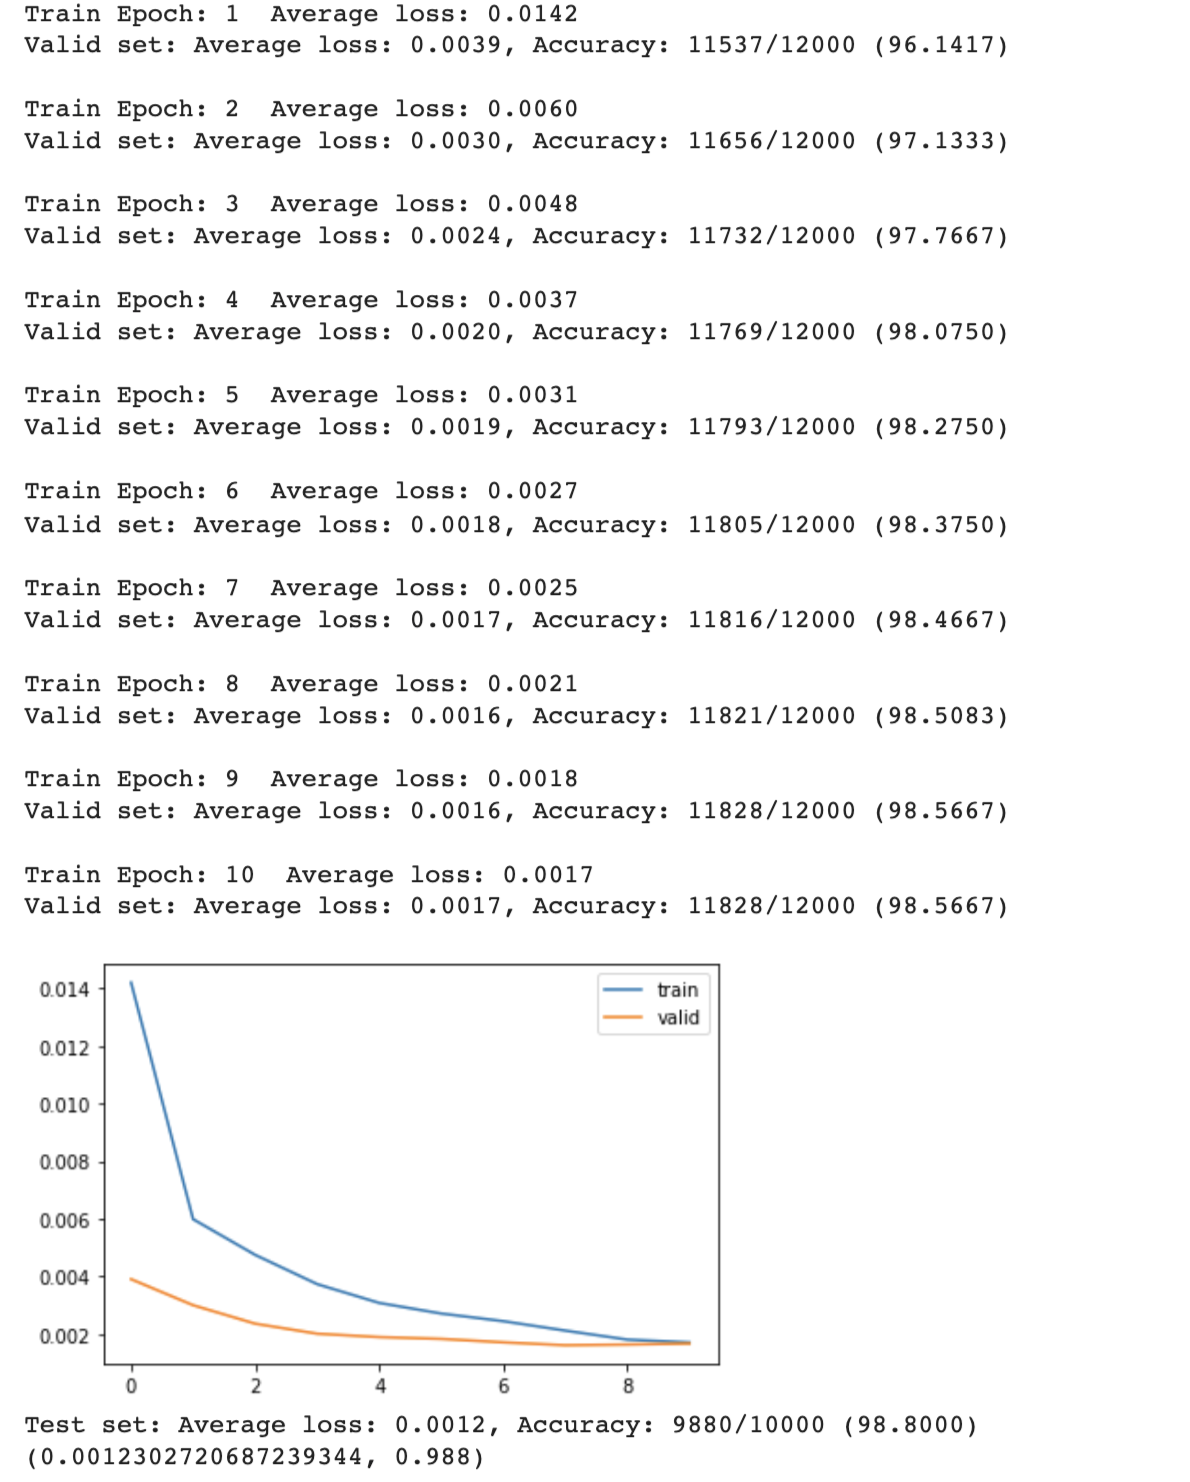
\includegraphics[scale=0.5]{convResults.png}
\end{center}
The first model I used worked using the default batch and epoch size.  I  stacked two of the default convolutional models together.
\end{itemize}
\pagebreak
\subsection{Problem III}
\begin{itemize}
\item[(a)]\begin{center}
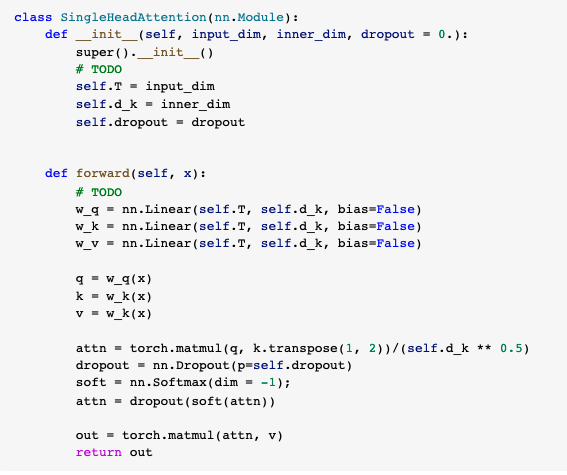
\includegraphics[scale=0.5]{single_head.png}
\end{center}
\item[(b)]
\begin{center}
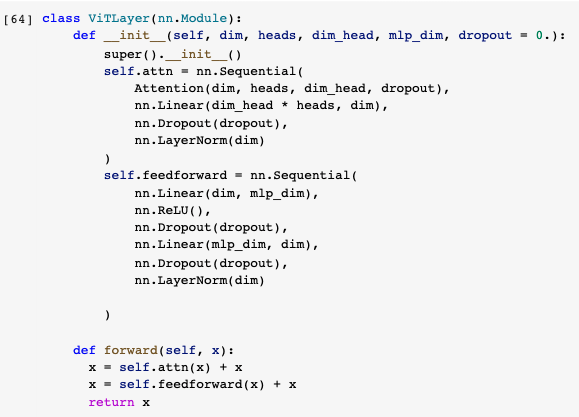
\includegraphics[scale=0.5]{vitlayer.png}
\end{center}
\item[(c)]\begin{center}
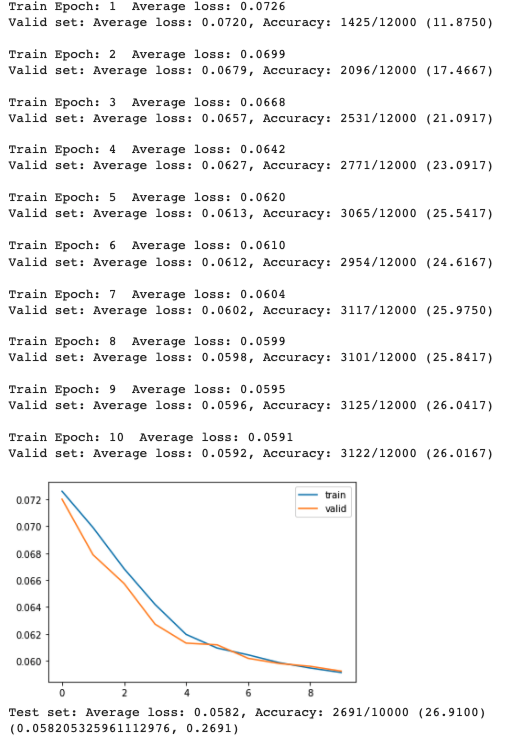
\includegraphics[scale=0.5]{2results.png}
\end{center}

\end{itemize}

\end{document}
